\hypertarget{CIstuff_8c}{
\section{CIstuff.c File Reference}
\label{CIstuff_8c}\index{CIstuff.c@{CIstuff.c}}
}
{\tt \#include \char`\"{}CI\_\-common.h\char`\"{}}\par


Include dependency graph for CIstuff.c:\begin{figure}[H]
\begin{center}
\leavevmode
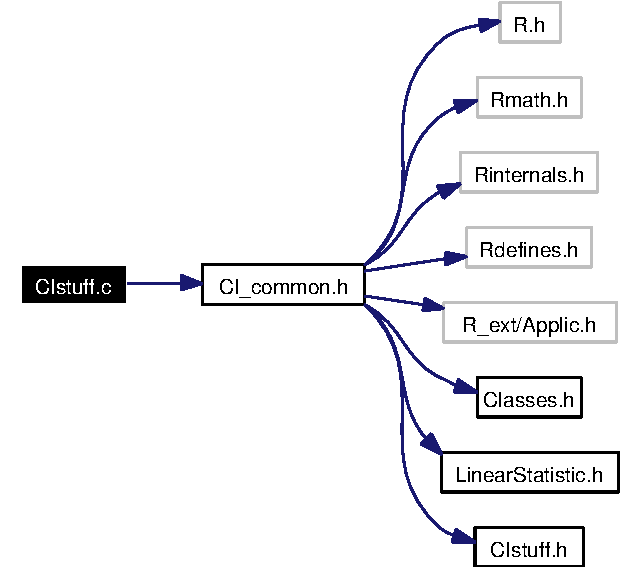
\includegraphics[width=165pt]{CIstuff_8c__incl}
\end{center}
\end{figure}
\subsection*{Functions}
\begin{CompactItemize}
\item 
int \hyperlink{CIstuff_8c_a0}{nrow} (SEXP x)
\item 
int \hyperlink{CIstuff_8c_a1}{ncol} (SEXP x)
\item 
void \hyperlink{CIstuff_8c_a2}{C\_\-Sample\-No\-Replace} (int $\ast$x, int m, int k, int $\ast$ans)
\item 
SEXP \hyperlink{CIstuff_8c_a3}{R\_\-blocksetup} (SEXP block)
\item 
void \hyperlink{CIstuff_8c_a4}{C\_\-blockperm} (SEXP blocksetup, int $\ast$ans)
\item 
SEXP \hyperlink{CIstuff_8c_a5}{R\_\-blockperm} (SEXP block)
\item 
SEXP \hyperlink{CIstuff_8c_a6}{R\_\-Monte\-Carlo\-Independence\-Test} (SEXP x, SEXP y, SEXP block, SEXP B)
\item 
SEXP \hyperlink{CIstuff_8c_a7}{R\_\-maxstattrafo} (SEXP x, SEXP cutpoints)
\end{CompactItemize}


\subsection{Detailed Description}
Some additional functionality for package `Conditional\-Inference'

\begin{Desc}
\item[Author:]\begin{Desc}
\item[Author]hothorn \end{Desc}
\end{Desc}
\begin{Desc}
\item[Date:]\begin{Desc}
\item[Date]2005/07/28 15:04:29 \end{Desc}
\end{Desc}


Definition in file \hyperlink{CIstuff_8c-source}{CIstuff.c}.

\subsection{Function Documentation}
\hypertarget{CIstuff_8c_a4}{
\index{CIstuff.c@{CIstuff.c}!C_blockperm@{C\_\-blockperm}}
\index{C_blockperm@{C\_\-blockperm}!CIstuff.c@{CIstuff.c}}
\subsubsection[C\_\-blockperm]{\setlength{\rightskip}{0pt plus 5cm}void C\_\-blockperm (SEXP {\em blocksetup}, int $\ast$ {\em ans})}}
\label{CIstuff_8c_a4}


Block permutation \begin{Desc}
\item[Parameters:]
\begin{description}
\item[{\em blocksetup}]as computed by `R\_\-blocksetup' \item[{\em ans}]integer vector \end{description}
\end{Desc}


Definition at line 96 of file CIstuff.c.

References C\_\-Sample\-No\-Replace().

Referenced by R\_\-blockperm(), and R\_\-Monte\-Carlo\-Independence\-Test().

Here is the call graph for this function:\begin{figure}[H]
\begin{center}
\leavevmode
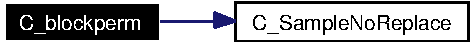
\includegraphics[width=130pt]{CIstuff_8c_a4_cgraph}
\end{center}
\end{figure}
\hypertarget{CIstuff_8c_a2}{
\index{CIstuff.c@{CIstuff.c}!C_SampleNoReplace@{C\_\-SampleNoReplace}}
\index{C_SampleNoReplace@{C\_\-SampleNoReplace}!CIstuff.c@{CIstuff.c}}
\subsubsection[C\_\-SampleNoReplace]{\setlength{\rightskip}{0pt plus 5cm}void C\_\-Sample\-No\-Replace (int $\ast$ {\em x}, int {\em m}, int {\em k}, int $\ast$ {\em ans})}}
\label{CIstuff_8c_a2}


compute a permutation of a (random subset of) 0:(m-1) \begin{Desc}
\item[Parameters:]
\begin{description}
\item[{\em x}]an integer vector of length m \item[{\em m}]integer \item[{\em k}]integer \item[{\em ans}]an integer vector of length k \end{description}
\end{Desc}


Definition at line 28 of file CIstuff.c.

Referenced by C\_\-blockperm().\hypertarget{CIstuff_8c_a1}{
\index{CIstuff.c@{CIstuff.c}!ncol@{ncol}}
\index{ncol@{ncol}!CIstuff.c@{CIstuff.c}}
\subsubsection[ncol]{\setlength{\rightskip}{0pt plus 5cm}int ncol (SEXP {\em x})}}
\label{CIstuff_8c_a1}




Definition at line 15 of file CIstuff.c.

Referenced by R\_\-Expect\-Covar\-Influence(), R\_\-Expect\-Covar\-Linear\-Statistic(), R\_\-Linear\-Statistic(), R\_\-Monte\-Carlo\-Independence\-Test(), and R\_\-Permuted\-Linear\-Statistic().\hypertarget{CIstuff_8c_a0}{
\index{CIstuff.c@{CIstuff.c}!nrow@{nrow}}
\index{nrow@{nrow}!CIstuff.c@{CIstuff.c}}
\subsubsection[nrow]{\setlength{\rightskip}{0pt plus 5cm}int nrow (SEXP {\em x})}}
\label{CIstuff_8c_a0}




Definition at line 11 of file CIstuff.c.

Referenced by R\_\-Expect\-Covar\-Influence(), R\_\-Expect\-Covar\-Linear\-Statistic(), R\_\-Linear\-Statistic(), R\_\-Monte\-Carlo\-Independence\-Test(), and R\_\-Permuted\-Linear\-Statistic().\hypertarget{CIstuff_8c_a5}{
\index{CIstuff.c@{CIstuff.c}!R_blockperm@{R\_\-blockperm}}
\index{R_blockperm@{R\_\-blockperm}!CIstuff.c@{CIstuff.c}}
\subsubsection[R\_\-blockperm]{\setlength{\rightskip}{0pt plus 5cm}SEXP R\_\-blockperm (SEXP {\em block})}}
\label{CIstuff_8c_a5}




Definition at line 125 of file CIstuff.c.

References C\_\-blockperm(), and R\_\-blocksetup().

Here is the call graph for this function:\begin{figure}[H]
\begin{center}
\leavevmode
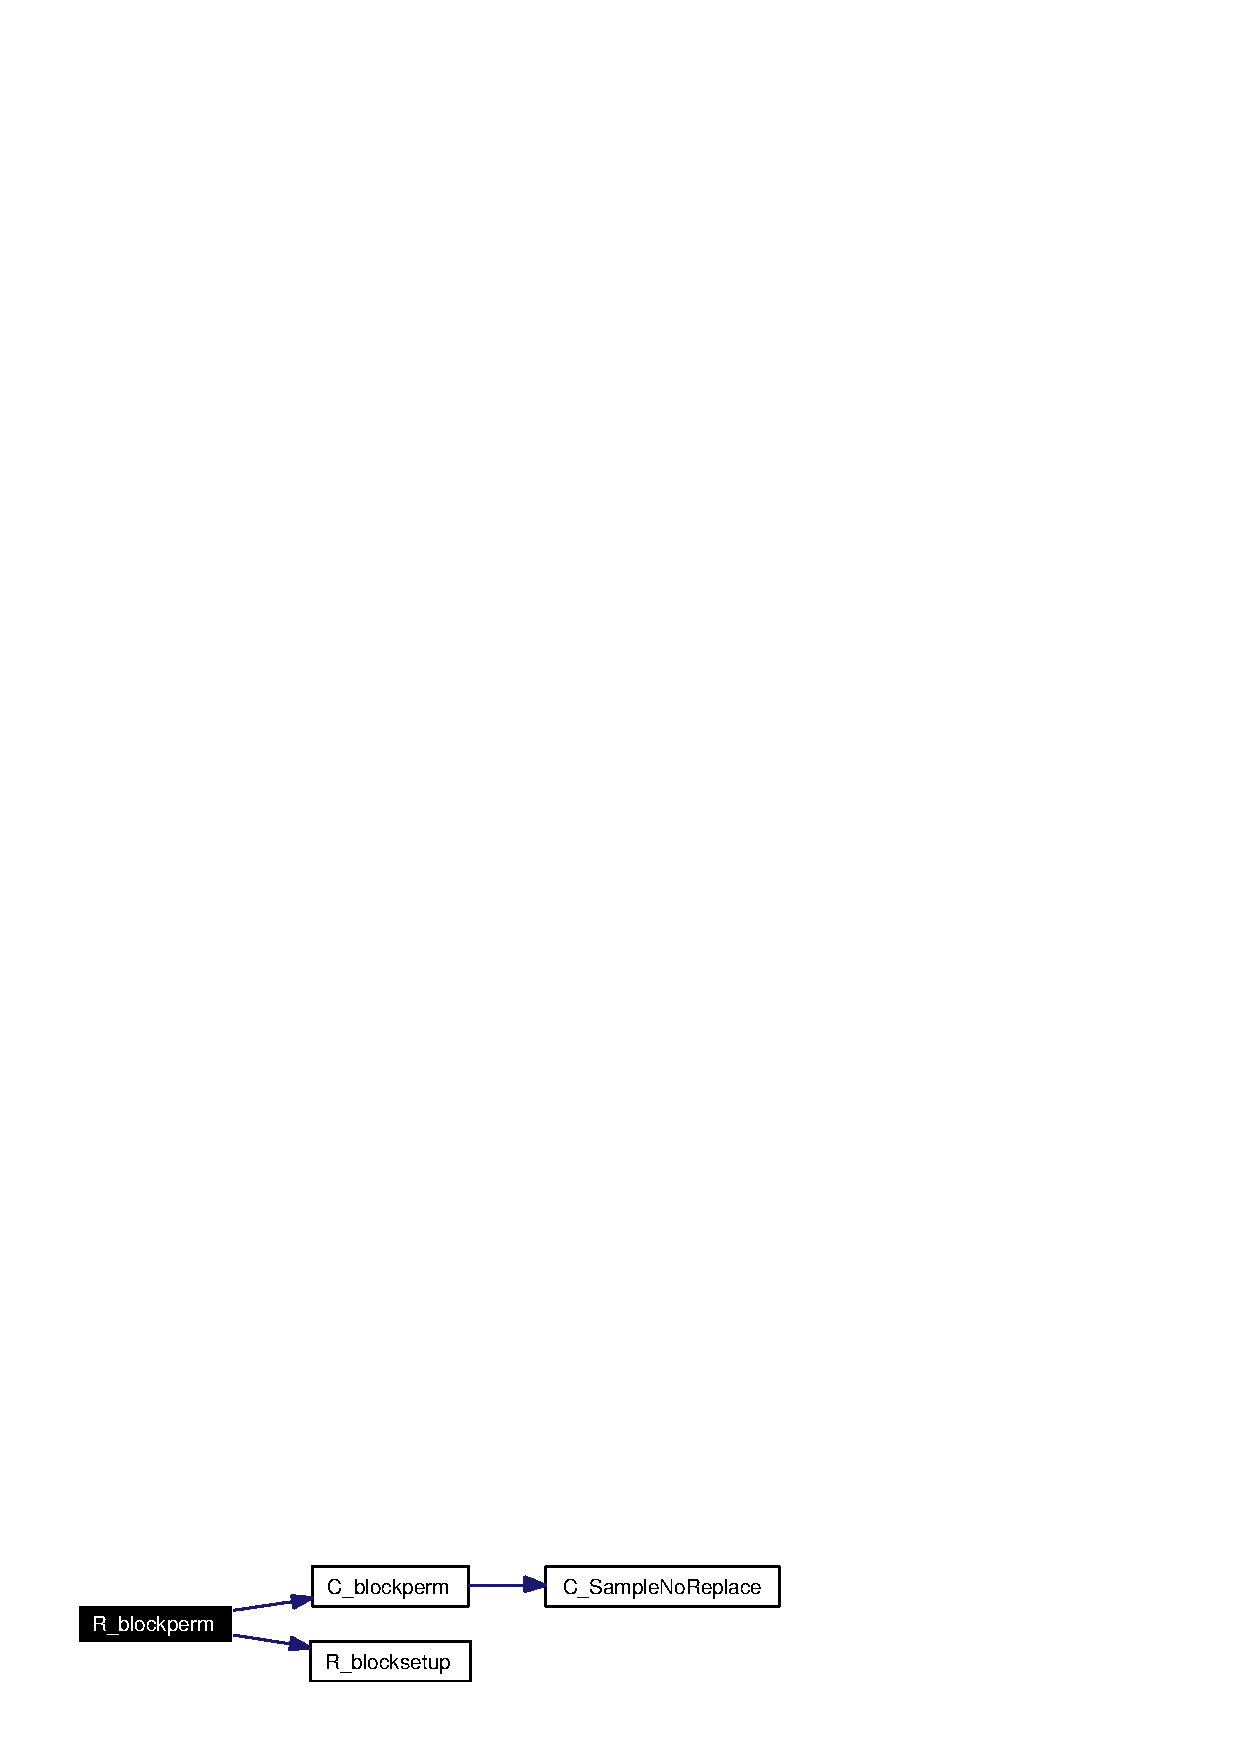
\includegraphics[width=187pt]{CIstuff_8c_a5_cgraph}
\end{center}
\end{figure}
\hypertarget{CIstuff_8c_a3}{
\index{CIstuff.c@{CIstuff.c}!R_blocksetup@{R\_\-blocksetup}}
\index{R_blocksetup@{R\_\-blocksetup}!CIstuff.c@{CIstuff.c}}
\subsubsection[R\_\-blocksetup]{\setlength{\rightskip}{0pt plus 5cm}SEXP R\_\-blocksetup (SEXP {\em block})}}
\label{CIstuff_8c_a3}




Definition at line 42 of file CIstuff.c.

Referenced by R\_\-blockperm(), and R\_\-Monte\-Carlo\-Independence\-Test().\hypertarget{CIstuff_8c_a7}{
\index{CIstuff.c@{CIstuff.c}!R_maxstattrafo@{R\_\-maxstattrafo}}
\index{R_maxstattrafo@{R\_\-maxstattrafo}!CIstuff.c@{CIstuff.c}}
\subsubsection[R\_\-maxstattrafo]{\setlength{\rightskip}{0pt plus 5cm}SEXP R\_\-maxstattrafo (SEXP {\em x}, SEXP {\em cutpoints})}}
\label{CIstuff_8c_a7}




Definition at line 184 of file CIstuff.c.\hypertarget{CIstuff_8c_a6}{
\index{CIstuff.c@{CIstuff.c}!R_MonteCarloIndependenceTest@{R\_\-MonteCarloIndependenceTest}}
\index{R_MonteCarloIndependenceTest@{R\_\-MonteCarloIndependenceTest}!CIstuff.c@{CIstuff.c}}
\subsubsection[R\_\-MonteCarloIndependenceTest]{\setlength{\rightskip}{0pt plus 5cm}SEXP R\_\-Monte\-Carlo\-Independence\-Test (SEXP {\em x}, SEXP {\em y}, SEXP {\em block}, SEXP {\em B})}}
\label{CIstuff_8c_a6}




Definition at line 138 of file CIstuff.c.

References C\_\-blockperm(), C\_\-Permuted\-Linear\-Statistic(), ncol(), nrow(), and R\_\-blocksetup().

Here is the call graph for this function:\begin{figure}[H]
\begin{center}
\leavevmode
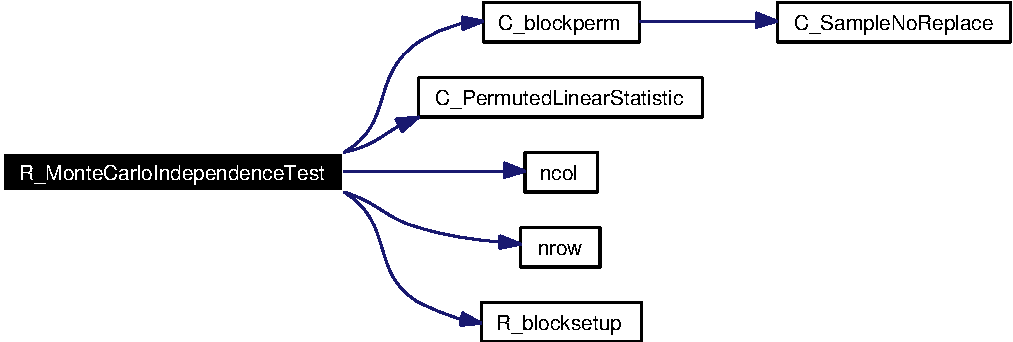
\includegraphics[width=260pt]{CIstuff_8c_a6_cgraph}
\end{center}
\end{figure}
